\documentclass[convert,float=false,crop=true]{standalone}
\usepackage{graphicx}
\usepackage{tikz}

\definecolor{tlpred}{RGB}{255,0,51}
\definecolor{tlpamber}{RGB}{255,192,0}
\definecolor{tlpgreen}{RGB}{51,255,0}
\definecolor{tlpwhite}{RGB}{255,255,255}

\begin{document}

  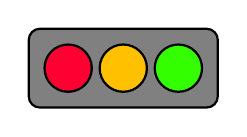
\begin{tikzpicture}[rounded corners, thick]
    %\shade[top color=yellow,bottom color=black] (0,0) rectangle +(2,1);
    %\shade[left color=yellow,right color=black] (3,0) rectangle +(2,1);
    %\shadedraw[inner color=yellow,outer color=black,draw=yellow] (6,0) rectangle +(2,1);
    %\shade[color=white] (0,3) rectangle +(1,1);
    %\shade[color=gray] (0,0) rectangle +(3,1);
    %\shade[ball color=green] (9,.5) circle (.5cm);

    %\foreach \x in {0,0.7,1.45} \draw (\x, 0) circle (0.3);
    \draw[fill=gray] (0,-0.5) rectangle +(2.4,1);
    \draw[fill=tlpred] (0.5, 0) circle (0.3);
    \draw[fill=tlpamber] (1.2, 0) circle (0.3);
    %\draw[fill=gray!80, color = gray] (1.2, 0) circle (0.3);
    \draw[fill=tlpgreen] (1.9, 0) circle (0.3);
    %\draw[fill=gray!80] (1.95, 0) circle (0.3);
  \end{tikzpicture}

\end{document}

https://www.cisa.gov/tlp
RGB:
TLP:RED : R=255, G=0, B=51, background: R=0, G=0, B=0
TLP:AMBER : R=255, G=192, B=0, background: R=0, G=0, B=0
TLP:GREEN : R=51, G=255, B=0, background: R=0, G=0, B=0
TLP:WHITE : R=255, G=255, B=255, background: R=0, G=0, B=0

CMYK:
TLP:RED : C=0, M=100, Y=79, K=0, background: C=0, M=0, Y=0, K=100
TLP:AMBER : C=0, M=25, Y=100, K=0, background: C=0, M=0, Y=0, K=100
TLP:GREEN : C=79, M=0, Y=100, K=0, background: C=0, M=0, Y=0, K=100
TLP:WHITE : C=0, M=0, Y=0, K=0, background: C=0, M=0, Y=0, K=100
